\documentclass[12pt]{report}

% Include all packages from file.
\usepackage[english]{babel}
\usepackage[utf8]{inputenc}
\usepackage{amsmath}
\usepackage{csquotes}% Recommended

\usepackage[a4paper,width=150mm,top=25mm,bottom=25mm]{geometry} %Paper margins
\usepackage{tikz}
\usetikzlibrary{calc}
\newcommand\HRule{\rule{\textwidth}{1pt}}

\usepackage[nolist,nohyperlinks]{acronym}

\usepackage{newtxtext,newtxmath}

\usepackage[comma,colon]{natbib}
\bibliographystyle{agsm}

\usepackage{hyperref}






\renewcommand{\contentsname}{Table of Contents}
\renewcommand{\baselinestretch}{1.5}

% HEADER AND FOOTER--------------------------
\patchcmd{\chapter}{\thispagestyle{plain}}{\thispagestyle{fancy}}{}{}
\pagestyle{fancy}
\fancyhf{}
\lhead{\fontsize{10}{12}\leavevmode\selectfont\color{gray}{Anomaly Detection \& Root Cause Analysis In Distributed Systems | Project Proposal}}
\rfoot{\fontsize{10}{12}\leavevmode\selectfont\color{gray}{\thepage}}
\lfoot{\fontsize{10}{12}\leavevmode\selectfont\color{gray}{Isala Piyarisi | 2018421}}
\renewcommand{\headrulewidth}{0pt}
% END HEADER AND FOOTER--------------------------


% Document begins here
\begin{document}

% TITLE PAGE---------------------------------------------------
\begin{titlepage}

\begin{tikzpicture}[remember picture, overlay]
  \draw[line width = 1pt] ($(current page.north west) + (1cm,-1cm)$) rectangle ($(current page.south east) + (-1cm,1cm)$);
\end{tikzpicture}

\begin{center}

% Upper part of the page
% \text{\large Informatics Institute of Technology}\\[0.1cm]
% \text{\large In Collaboration With}\\[0.5cm]
% \text{\large University of Westminster, UK}\\[2.5cm]

% Title

\includegraphics[width=5.0cm]{assets/IIT-Logo.png}\\[0.7cm]
{ \Huge Anomaly Detection \& Root Cause Analysis\\
In Distributed Systems }\\[0.7cm]
% \begin{minipage}{0.45\textwidth}
\text{\LARGE  Project Specifications Design and Prototype}\\[0.5cm]

% Authors
% \text{\large A dissertation by}\\[0.1cm]
\text{\large Isala Piyarisi}\\[0.1cm]
\text{\large w1742118 / 2018421}\\[3.2cm]

% Supervisor
\text{\large \textbf{Supervisor}: Guhanathan Poravi}\\[0.1cm]
\text{\large \textbf{Date}: $13^{rd} $ February 2022}\\[0.1cm]
\text{\large \textbf{Department}: Computer Science}\\[0.1cm]
\text{\large \textbf{Keywords}: Cloud Computing, AIOps, Monitoring, Disaster Recovery}\\[5cm]


\large{Submitted in partial fulfilment of the requirements for the \\
BSc(Hons) Computer Science degree at the \\
University of Westminster.
} \\[0.5cm]


\end{center}

\end{titlepage} 

% Page Numbering---------------------------------------------
\pagenumbering{Roman}

% Table of Contents---------------------------------------------------
\tableofcontents
% List of Figures---------------------------------------------------
\addcontentsline{toc}{chapter}{\listfigurename}
\listoffigures
% List of Tables---------------------------------------------------
\addcontentsline{toc}{chapter}{\listtablename}
{\let\clearpage\relax 
\listoftables
}
\cleardoublepage
\phantomsection
% Include acronyms
\addcontentsline{toc}{chapter}{List of Acronyms}
% \acrodef{acronym}[short name]{full name}
\acrodef{IC}[IC]{Integrated Circuit}
% \acrodef{svm}[SVM]{Support Vector Machine}
\newacro{svm}[SVM]{Support Vector Machine}
% Example use \ac{IC} for printing "Integrated Circuit (IC), use \ac{IC} again and it will print (IC)"
% For plural use \acp{IC} for short and \aclp{IC} for long.
% For more see: http://ftp.acc.umu.se/mirror/CTAN/macros/latex/contrib/acronym/acronym.pdf

\section{Introduction}

There was a big shift towards cloud computing in recent years due to its scalability and  ease of use. With this change, a new programming paradigm called cloud-native was born. Cloud-native applications are often developed as a set of stand-alone microservices \citep{dragoni2017microservices} yet could depend on each other to provide a unified experience. This helps different teams to work on different services which increases the development velocity. This works well for medium to large companies but over time when this mesh of services could become very complicated to a point where it's very difficult for one person to understand the whole system.

When the system consists of 1000s of individual services talking and depending on each other, the network layer of that system becomes chaotic \citep{Introduc54:online} and failure in a single point can create a ripple effect across the system. When something like that happens it's really difficult to zero in on the exact point of failure quickly. In this research, I am planning to introduce a system that monitors all the services and detects if the service is acting out of shape and if so find the root cause of it by evaluating it on a dependency tree.
\pagenumbering{arabic}


{\let\clearpage\relax \chapter{Background}}

\section{Cloud Computing}
With an emergence \ac{iaas} like Amazon Web Services (AWS) and Google Cloud Platform (GCP) there is a big surge in organizations trying to outsource their computing needs to third parties \citep{rimol_2021}. This is mainly due to the elasticity given by all the cloud providers. Users can easily scale up and down their infrastructures within minutes without making any commitment and all the major providers, bill users on what you use are what you pay model because cloud provider manages all the underlying infrastructure users doesn't have to worry about problems like hardware failures. In contrast in a self-hosted setting if the user wanted one extra GB of memory than what's available it requires a lot of effort and cost to full fill that requirement.

\section{Cloud-Native Applications}
During the 90s and early 2000s, all the applications were made as a big monolith from a single code base. Most of them were shipped as a single binary. Since those days applications were fairly simple this worked very well with little to no downsides. But when the 2010s came around there were a lot of specialized frameworks and programming languages and marketing teams wanted a lot of new futures quickly developed still maintaining reliability. But if the code base of the application was stored in a single repository, developers have to go through a long process to review and test if the changes won't break the current system and developers are also limited by the framework and programming language initial develops chosen for the project.

To tackle these problems there was a new way to develop applications was introduced, it's called "Microservices". The idea behind this concept is to break all the functionalities of big monolith applications into small individually scalable services and give ownership of each service to small teams of people who work separately. With this flow developers are free to use whatever tool they like to develop each service. Because these services are developed parallelly by different teams this increases the development velocity by order of magnitude. \citep{Understa56:online}

As these services are relatively small and tailor-made to run on cloud environments it's very easy to take something that's running on the developer's local machine to the production cluster in a matter of minutes. This is mainly thanks to modern cloud-native tools like CI/CD pipelines which automatically build and test the code for them, which can save a lot of time spent just doing repetitive tasks which are prone to human errors. \citep{Whataret68:online}

\section{Monitoring Cloud-Native Applications} \label{monitoring-bg}
Even though cloud-native applications have a lot to offer when it comes to developer velocity and productivity, It has its fair share of issues. Most of these problems are linked to the sheer complexity of these systems and not having a proper way to monitor them \citep{5WaysYou35:online}. All 3 major cloud providers provide a way to monitor these applications efficiently and some great open-source projects do this well, But to take full advantage of those systems, developers have to adapt their services to export all the vitals in a way the monitoring system understand. This works for the most part and this is what all the big companies are doing, even if it takes more developer time to in the end it's very crucial when it comes to disaster recovery.

But there is still a slight problem with this approach. Once the system starts to scale up to 100s of services number vitals that has to be monitored goes to 1000s and will require a lot of additional \acp{sres} and will have drop lot of non-crucial service vitals and derive abstract \acp{sli} to make it \textbf{humanly} possible to understand what's going on.

\section{Problem Domain}

\section{Problem Definition}

\subsection{Problem Statement}


\section{Research Motivation}


{\let\clearpage\relax\chapter{Existing Work}}

\section{Anomaly detection}

% \setlength\LTleft{-5mm}

% \begin{longtable}{| p{20mm} | p{47mm} | p{47mm} | p{47mm} |}
\begin{longtable}{| p{20mm} | p{43mm} | p{43mm} | p{43mm} |}
\hline
  \textbf{Citation} &
  \textbf{Technology summary} &
  \textbf{Improvements} &
  \textbf{Limitations} \\ \hline
  \cite{du2018anomaly} &
  Tested most of common machine learning methods to detect anomalies and benchmarked them &
  \vspace{-8mm}
  \begin{itemize}[leftmargin=*,noitemsep,nolistsep] 
    \item Used SLIs to monitored data
    \item A lot of good metrics (input data)
    \item Performance monitoring of services and containers
  \vspace{-7mm}
  \end{itemize} &
  \vspace{-8mm}
  \begin{itemize}[leftmargin=*,noitemsep,nolistsep] 
    \item Only be able to identify predetermined issues
    \item Require a sidecar that includes a lot of overhead
    \item Won't work with event-driven architectures (this is where most of the new systems are headed)
    \item Uses Supervised learning and it's near impossible to find real-world data with labels
  \vspace{-7mm}
  \end{itemize} \\ \hline
  \cite{kumarage2018anomaly} &
  The authors here are proposing a semi-supervised technique using a Variational Autoencoder to predict future time steps and calculate the difference between predicted and actual to detect anomalies. &
  \vspace{-8mm}
  \begin{itemize}[leftmargin=*,noitemsep,nolistsep] 
    \item Due to the difficulty of finding labeled research data, they settled on using a semi-supervised technique.
    \item Used randomized decision trees were utilized to select the most suitable features for each component.
  \vspace{-7mm}
  \end{itemize} &
  \vspace{-8mm}
  \begin{itemize}[leftmargin=*,noitemsep,nolistsep] 
    \item The model won't be easily transformable for other systems
    \item If more new key features were added to the system it will require a total retraining
  \vspace{-7mm}
  \end{itemize} \\ \hline
  \cite{kumarage2019generative} &
  Uses a bidirectional GAN to predict future timesteps and uses MSE between prediction and real to determine the anomalies &
  Experimented using a GAN to detect anomalies rather than using conventional autoencoders &
  \vspace{-8mm}
  \begin{itemize}[leftmargin=*,noitemsep,nolistsep] 
    \item Accuracy is around 60% which is not really good to use in production with mission-critical systems.
    \item As this is a GAN-based system, it may take a lot of resources to run with production systems.
  \end{itemize} \\ \hline
  \caption{Comparison of anomaly detection methods in distributed systems}
\end{longtable}

\section{Root cause identification}

% \begin{longtable}{| p{20mm} | p{47mm} | p{47mm} | p{47mm} |}
\begin{longtable}{| p{20mm} | p{43mm} | p{43mm} | p{43mm} |}
\hline
  \textbf{Citation} &
  \textbf{Technology summary} &
  \textbf{Improvements} &
  \textbf{Limitations} \\ \hline
  \cite{gonzalez2017root} &
  Detect failures in networks, using machine learning to generate knowledge graphs on historical data &
  \vspace{-8mm}
  \begin{itemize}[leftmargin=*,noitemsep,nolistsep] 
    \item Build a predictable system
    \item Automatic identification of dependencies between system events
    \item Doesn't Need to rely on Domain experts
    \item Generalized to different systems
  \vspace{-7mm}
  \end{itemize} &
  \vspace{-8mm}
  \begin{itemize}[leftmargin=*,noitemsep,nolistsep] 
    \item Limited to network issues
    \item Even though the knowledge graph helped with visualization of the problem but still, people have to manually figure out what went wrong
  \vspace{-7mm}
  \end{itemize} \\ \hline
  \cite{chigurupati2017root} &
  Proposed a way to detect Hardware failures in servers using a probabilistic graphical model which concisely describes the relationship between many random variables and their conditional independence &
  \vspace{-8mm}
  \begin{itemize}[leftmargin=*,noitemsep,nolistsep] 
    \item Find hidden meaning in values that seems random
    \item Used a probabilistic approach to better understand the relationship between inputs and outputs
    \item Gives all the possible root cause to a given problem
  \vspace{-7mm}
  \end{itemize} &
  \vspace{-8mm}
  \begin{itemize}[leftmargin=*,noitemsep,nolistsep] 
    \item Limited to hardware issues
    \item Require support from domain experts
    \item Can't account for unforeseen error
  \vspace{-7mm}
  \end{itemize} \\ \hline
  \cite{samir2019dla} &
  This detects and locates the anomalous behavior of microservices based on the observed response time using a \ac{hhmm} &
  \vspace{-8mm}
  \begin{itemize}[leftmargin=*,noitemsep,nolistsep] 
    \item Custom HHMM model
    \item Self-healing mechanism
    \item Focus on performance detection and identification at the container, node, and microservice level
  \vspace{-7mm}
  \end{itemize} &
  \vspace{-8mm}
  \begin{itemize}[leftmargin=*,noitemsep,nolistsep] 
    \item Input dataset scale is limited
    \item Require a sidecar
    \item Needs to predetermined thresholds
  \vspace{-7mm}
  \end{itemize} \\ \hline
  \cite{wu2020microrca} &
  Find Performance bottlenecks in distributed systems using an attribute graph to find anomaly propagation across services and machines &
  \vspace{-8mm}
  \begin{itemize}[leftmargin=*,noitemsep,nolistsep] 
    \item Created a custom Faults Injection module
    \item Uses an attribute graph to localize to faulty service
    \item Application-agnostic by using a service mesh
    \item Rely on service mesh to determine network topology
    \item Uses unsupervised learning
  \vspace{-7mm}
  \end{itemize} &
  \vspace{-8mm}
  \begin{itemize}[leftmargin=*,noitemsep,nolistsep] 
    \item Only able to identify 3 types of issues
    \item Looks only for performance anomalies
    \item Use the slow response time of a microservice as the definition of an anomaly
    \item Service meshes add a lot of overhead to systems
    \item Required direct connection between services
  \vspace{-7mm}
  \end{itemize} \\ \hline
  \caption{Comparison of root cause identification methods in distributed systems}
\end{longtable}

% \newpage
\section{Commercial products}

% \begin{longtable}{| p{40mm} | p{60mm} | p{60mm} |}
\begin{longtable}{| p{40mm} | p{55mm} | p{55mm} |}
\hline
  \textbf{Name} &
  \textbf{Futures} &
  \textbf{Limitations} \\ \hline
  Applied Intelligence by New Relic &
  \vspace{-8mm}
  \begin{itemize}[leftmargin=*,noitemsep,nolistsep] 
    \item Metric forecasting.
    \item Anomaly detection.
    \item Alert grouping to reduce noise.
  \vspace{-7mm}
  \end{itemize} &
  \vspace{-8mm}
  \begin{itemize}[leftmargin=*,noitemsep,nolistsep] 
    \item Lack of explainability for certain classifications.
    \item All the telemetry data need to be sent to a third party.
  \vspace{-7mm}
  \end{itemize} \\ \hline
  Watchdog by Datadog &
  \vspace{-8mm}
  \begin{itemize}[leftmargin=*,noitemsep,nolistsep] 
    \item Monitor the metric data of the entire system from the background.
    \item Monitor logging data.
    \item Highlight relevant components affected by an issue.
  \vspace{-7mm}
  \end{itemize} &
  \vspace{-8mm}
  \begin{itemize}[leftmargin=*,noitemsep,nolistsep] 
    \item Announced in 2018 but is still at private beta.
    \item Require code changes and tight integration with datadog platform.
    \item Available demos about the system seems to be engineered for demonstration purposes.
  \vspace{-7mm}
  \end{itemize} \\ \hline
  \caption{Comparison of commercial products for root cause analysis}
\end{longtable}
% \setlength\LTleft{5mm}
% As the large-scale migration towards the cloud and microservices started fairly recently the problem this research is trying to solve mostly affects large-scale enterprises there ain't a lot of published research on this domain. All the work done towards uncovering the root cause of failures by large co-operations either kept their finds for internal use to sell it as \ac{saas} product. 

% One of the best implementations found on root cause analysis is from Datadog. They created a platform called watchdog \citep{Watchdog76:online} which monitors the entire system for anomalies and failures in the background. When a failure happens it tries to pull all the relevant stack traces and monitoring data to a single view so the developer can diagnose the problem easily. The problem with this solution is even though it was announced all the way back in July 2018, all that is available is currently in private beta which not everyone has access to.
% \\
% All the currently published work on microservices monitoring can be classified into 2 categories
% \begin{enumerate}
% \item Anomaly detection
% \item Root cause identification
% \end{enumerate}

% \section{Anomaly detection}

% Anomaly detection in time series is a field of its own. So in this case we will be forcing papers that are specialized in the cloud computing domain.

% One of the earliest attempts on detecting anomalies in microservices was \cite{du2018anomaly}. In this authors tried using 4 different machine learning techniques to detect performance anomalies. To do this say used a simulated system and various fault injection mechanisms to create the dataset. In the end, they concluded K Nearest Neighbors classifier gives the most accurate classifications while Support vector machines have the worse.

% A common way to detect anomalies in time series is using an autoencoder to reconstruct a given time series. After training the model should be able to come up with the generalized function about the given time series and it will be able to recreate any input sequence accurately. But when there is an anomaly in the input sequence models output will be vastly different from the input. We can use this reconstruction loss as a metric to uncover anomalies within the system. In \cite{kumarage2018anomaly} authors used the method to detect anomalies in distributed systems. In a continuation of their work \cite{kumarage2019generative} they tried doing the same thing by using a GAN but in the end, they concluded even though it showed a tendency towards better performance when the dataset gets bigger, with the dataset they had autoencoders perform well overall.

% Ever since DeepMind came up with wavenet which used a CNN to generate audio samples \citep{oord2016wavenet} researchers uncovering other potential use cases other than image-related tasks. One of those use cases was as CNN excels at pattern recognition, encoding time series data set into image-like data structures and use a CNN to identify abnormal patterns in it. On \cite{kim2018encoding} authors tried to using a novel technique to raw encode data into a pixel-like structure and found it could outperform the existing methods to detect anomalies in computer networks.

% \section{Root cause identification}

% Predicting the exact root cause of failure just using a standard machine learning model is a pretty difficult task since prediction space is not finite. In 2017 a team from Google X tried using the Bayesian Network to model the relationship between the state of the system and its effect on failures \citep{chigurupati2017root}. Using it they were able to accurately predict all the possible root causes of a hardware failure in certain systems but this model required to predefine all the possible error modes by domain experts which isn't really possible in a constantly evolving distributed system. There were similar attempts \cite{gonzalez2017root} to use machine learning to generate knowledge graphs on historical data and help developers come up with reasoning to failures although this eliminated a need for a domain expert, this also can't react to unseen errors.

% In a distributed system it's hard to spot real anomalies just by looking at monitoring data, but when there are huge spikes in response latencies or error rates it's a good indicator something must be wrong. So \cite{samir2019dla} used a \ac{hhmm} to uncover the possible affected services from changes in response time or error rates in one service and using that data to uncover the root cause of the issue. All of the papers discussed above have one problem in common they all assume the entire system is static but in reality, these services changes over time either with increased demand or new future implementations. To address this, \cite{wu2020microrca} developed a service that monitors all the running applications and their vitals. This also constructs an attributed graph that represents how each service interacts with the other. When the monitoring system detects an anomaly MicroRCA weight that graph with response time changes and tries to find the epicenter of the anomaly. The main problem with both of these approaches have is authors rely solely on slow response time as an indication of an anomaly but several other factors could course anomalous behaviors without changes in response times.


{\let\clearpage\relax\chapter{Research Gap}}

After a literature survey author came conclusion finding a root cause of any failure within a distributed system is a very difficult issue due to it not having single output we can try to predict and most researchers have built their own simulation of a distributed system by themselves since there isn't any open dataset about monitoring data mainly because it could contain sensitive information. 

Most currently established researches are done towards creating statistical models like clustering and linear regression. Even though these algorithms perform very well in small-scale systems, they struggle to keep up when the monitoring data become very noisy with scale. Another problem none of these papers properly  addressed was constant changes to services. All most published research considers target services as static but in reality, these services can change even many times per day \citep{GoingtoM51:online}.

After talking with industry experts author concluded three main issues all had with using a machine learning model as monitoring agent Reliability, Interpretability, and Tunability. On reliability, experts said too many false positives will make operators lose faith in the system because it's gonna be another distraction to them. As the operators have to take critical decisions with the output of these models, it has been interpretable by humans \citep{ribeiro2016should}. Finally, this system should act more like a tool rather than a replacement to human operators, because no matter machine learning models cannot compete with the context a human can handle. 

\section{Research Contribution}

With this research the author first try to develop a cloud-native solution to create a configurable microservices system, So this research and future researches will have a standard environment develop and evaluate their work.
\label{need-for-encoding}
Another problem with monitoring microservices systems is different services can be developed with different programming languages and frameworks and those can contain different levels of noisiness. So it's hard for a single model to detect anomalies in any service since some frameworks tend to use more resources while idle than others.  So to address this author is trying to come up with an encoding method so the model can be trained to monitor one framework and those learning will still be valid for another framework.

With those encoded data the author are hoping to develop a convolutional autoencoder that will use unsupervised learning to spot out anomalies in a given data stream. This may have better performance while using fewer resources convolutional layers are typically lightweight and good at pattern recognition \citep{oord2016wavenet}.

Finally, the author is planning to aggregate those predictions from the models into a pre-generated service graph and weigh it to give possible root causes.


{\let\clearpage\relax\chapter{Research Challenge}}

Even though this project seems very straightforward and easy to implement from a high level, but it becomes tricky when attempting to reach targets defined in section \ref{sec:in-scope}.
\\
\begin{itemize}[leftmargin=*] 
\item \textbf{Highly seasonal and noisy patterns} - Monitoring metrics on microservices on production tends to have very unpredictable patterns depending on the traffic that's sent to the service. The amount of traffic sent will depend on several external factors that are hard to determine. Modeling both temporal dependencies and interdependencies between monitoring data into a single graph will be very difficult and require a lot of fine-tuning and data engineering.
\item \textbf{Overhead} - Modern deep learning models can solve any problem if we could give it an unlimited amount of data and processing power but In this case, models need to optimize for efficiency over accuracy since having a monitoring system that consumes a lot more resource than the actual target system isn't effective.
\item \textbf{Fit into Kubernetes eco-system} - Kubernetes has become the de-facto standard to managing distributed systems \citep{WhatisCo78:online}. So the author is planning to create a Kubernetes extension that will bridge the connection between monitored service and monitoring model as shown in the figure \ref{fig:high-level-diagram}. But Kubernetes itself has a very steep learning curve, even the original developers themselves admitted it's too hard complex for beginners \cite{Googlead4:online}.
\end{itemize}

\section{Research Question}


\begin{enumerate}[leftmargin=*,label=\textbf{RQ\arabic*:}]

\item Can encoding raw data monitoring into an image-like structure can improve the performance of autoencoders?

\item Is it possible for a single machine learning model to extract the underlying function in all of the monitoring data of a microservice?

\item  Can the model me generalize enough so, with few-shot learning, the same model can be set to predict anomalies in a completely different service?

\item Can a weighted graph on anomaly scores be used to predict a root cause of a failure?

\item Can reinforcement learning be applied here so the model is continuously adapting to changes done to host service?

\end{enumerate}



\section{Achievement of Research Aims \& Objectives}

\subsection{Aim of the Project}

\section{Research Aim}

\textit{The aim of this research is to design, develop and evaluate a low overhead Kubernetes framework to collect, store and process telemetry data using deep learning to help system operators detect anomalies earlier in order to reduce the \ac{mttr} when the system is experiencing an anomaly.}

The aim of the project was successfully achieved by designing, developing, and evaluating a flexible framework which made the components interchangeable. This makes it easy for the data scientist to create reliable machine learning models to find the root causes of anomalies, which in turn help the system operators to reduce the \ac{mttr}.


\subsection{Research Objectives}

\begin{longtable}{|p{40mm}|p{91mm}|p{20mm}|}
    \hline
    \textbf{Research Objective} & \textbf{Justification} & \textbf{Status} \\ \hline
    Problem identification & A project with proper scope was identified to research on. & Completed \\ \hline
    Literature review & A detailed literature survey was conducted on all related topics. & Completed \\ \hline
    Developing an evaluation framework & \href{https://github.com/MrSupiri/MicroSim}{MicroSim} was developed and published. & Completed \\ \hline
    Data gathering and analysis & \ac{ebpf} agent \ac{gazer} and data preprocessor \ac{sherlock} was developed. & Completed \\ \hline
    Developing encoding methods & \ac{sherlock} uses the RGB colour scheme to represent the telemetry data. & Completed \\ \hline
    Developing the model & An autoencoder was developed to detect anomalies. & Completed \\ \hline
    Testing and evaluation & Both functional and non-functional tests were carried out to verify the capabilities of the project. Along with third party evaluation. & Completed \\ \hline
    Integration & \ac{lazy-koala-operator} was built to bind up all the components together. & Completed \\ \hline
    \caption{Achievements of Research Objectives(self-composed)}
  \end{longtable}
  
  

{\let\clearpage\relax\chapter{Research Objectives}}

\newcommand\robProblemIdentification{
When selecting the problem author wanted to pursue, they had 3 main goals.
\begin{enumerate}[leftmargin=*,noitemsep,nolistsep] 
\item The problem domain should be something they enjoy working in.
\item At the end of the research should have done a meaningful impact on the target domain, both in the theoretical and practical aspect,
\item It should be challenging to achieve and results should speak about themselves.
\end{enumerate}
% After many iterations of trial and error the author settled on "Cloud Computing" as the domain, "Root cause analysis" as the problem because the author is a site reliability engineer by profession and quickly able to identifying the root cause of a failure could lower \ac{mttr}.
}

\newcommand\robLiteratureReview{
% After a general topic was identified, the author needed to do evaluate all the currently published work to understand what’s the current state of the problem and how other researchers and developers are approaching this problem. After an intensive literature survey author was able to identify a new angle to approach the domain.

% During this period author contacted few experts in the cloud computing domain and evaluate the idea and plan for the project.
Conduct a Literature review on root cause analysis to, 
\begin{itemize}[leftmargin=*,noitemsep,nolistsep] 
\item To find the current methods used to anomaly detection and localization.
\item Uncover issues with current approaches.
\item Understand how advancement in other related domains can apply to this domain.
\end{itemize}
}


\newcommand\robDevelopingEvaluation{
During the literature survey, one problem the author identified was there isn’t a uniform dataset when it comes to training and evaluating models to detect anomalies in microservices. Most of the researchers used private datasets to train and test their work.
To address this author is developing,
\begin{itemize}[leftmargin=*,noitemsep,nolistsep] 
\item A tool that can easily simulate a distributed system in a cloud-native setting.
\item A tool inject anomalies into the running services.
\end{itemize}
}

\newcommand\robPublishPlayground{
The author is hoping to publish a paper about the above-mentioned tool so the future researchers will have a unified way to train, test, and benchmark their system without having to reinvent the wheel again and again.
}

\newcommand\robDataGathering{
% The author plans to use the above-mentioned tool to simulate a large-scale distributed system made up of services done in different frameworks and subject it to a load test. Then collect the monitoring data from that to train the model.
In order to create model to detect anomalies the author will,
\begin{itemize}[leftmargin=*,noitemsep,nolistsep] 
\item Simulate distributed system.
\item Simulate traffic inside the system
\item Collect monitoring data while it's running
\end{itemize}
}

\newcommand\robDevelopingEncoding{
As mentioned in the section \ref{need-for-encoding} these services will report very different values even at idle. To normalize data from all the services to one format author will,
\begin{itemize}[leftmargin=*,noitemsep,nolistsep] 
\item Evaluate current data encoding methods like \cite{zhang2019deep}.
\item Find the best one fit and optimize it to this use case.
\item Test if there is any improvement by using this method. 
\end{itemize}

% So there needs to be a way to normalize data from all the services to one format so the model can generalize for all the services no matter the framework it was built on. Inspired by \cite{zhang2019deep} the author is trying to develop or adopt an encoding technique to present data in an image-like structure so both ML models and humans can spot out anomalies easily.
}


\newcommand\robDevelopingModel{
% Autoencoders have been outperforming all other types of models \citep{kumarage2019generative} when it comes to anomaly detection. Since this project already has a module that converts raw data to an image-like structure the author is hoping to use a convolution autoencoder which will be lighter and has the potential to outperform normal autoencoders when paired with the above data encoding technique.
According to \cite{kumarage2019generative} Autoencoders tend to perform best when it comes to anomaly detection. But during the literature survey it was raveled Conversational Autoencoders weren't tested. So author tries to develop a  Conversational Autoencoders and test how it will perform.
}


\newcommand\robTesting{
Following things will be tested during the testing phase, 
\begin{itemize}[leftmargin=*,noitemsep,nolistsep] 
\item How will the system classify long-term fluctuations.
\item How will the system classify short-term fluctuations.
\item Can the system understand the mapping between core metrics like CPU and Memory usages.
\item Accuracy of fault detection.
\item Accuracy of root cause localization.
\end{itemize}
% The author hopes to carry an extensive evaluation on the system with a wide variety of edge cases and the author is hoping to see how the model identifies both short-term and long-term fluctuations and whether it can properly find a mapping between core vitals like CPU and Memory usages.
}


\newcommand\robIntegration{
Having a fancy model doesn’t add means anything if it’s very hard to use in a real system. So the author is hoping to develop a Kubernetes extension that will map the model with any service given by the user.
}


% \begin{table}[]
\begin{longtable}{|p{3cm}|p{10cm}|p{1.5cm}|}
\hline
\textbf{Research Objectives}          & \textbf{Explanation}      & \textbf{Learning Outcome} \\ \hline
Problem identification                & \robProblemIdentification & LO1                       \\ \hline
Literature review                     & \robLiteratureReview      & LO3, LO4, LO6             \\ \hline
Developing an evaluation framework    & \robDevelopingEvaluation  & LO7                       \\ \hline
Publish a paper about that playground & \robPublishPlayground     & LO7                       \\ \hline
Data gathering and analysis           & \robDataGathering         & LO7                       \\ \hline
Developing encoding method            & \robDevelopingEncoding    & LO2, LO5, LO7             \\ \hline
Developing the model                  & \robDevelopingModel       & LO2, LO5, LO7             \\ \hline
Testing and evaluation                & \robTesting               & LO8, LO9                  \\ \hline
Integration                           & \robIntegration           & LO7                       \\ \hline
\caption{Research Objectives}
\end{longtable}
% \end{table}
% \subsection{Project Objectives}
% \begin{itemize}
% \item Find area I am interested in
% \item Find a issue in it
% \item Evaluate the issue with experts in the field
% \item Create PID
% \item Create playground to test the final product in
% \item Publish a paper about that playground
% \item Finalize on requirements
% \item Develop prototype and Document the progress 
% \item Create operator to plugin any ML model to monitor
% \item Publish paper with results
% \item complete thesis
% \item conclude the project
% \item open source the code
% \end{itemize}

% \subsection{Research Objectives}
% \begin{itemize}
% \item Literature Survey
% \item Requirement Analysis
% \item Design
% \item Development
% \item Testing
% \end{itemize}

{\let\clearpage\relax\chapter{Project Scope}}

From the literature survey and talking with industry, experts author found many issues they can address when developing the system, but some of those problems like interpretability on autoencoder \citep{ribeiro2016should} are hard to solve by someone at a level of an undergraduate. As this project is done by one developer in less than one year, it won't be possible to create a fully functional monitoring platform like Datadog or New Relic. The Force of this project is to see if the author can develop a single model that can monitor all kinds of services after transfer learning with few examples. 

\section{In-scope} \label{sec:in-scope}
Following are the main forces of this project
\begin{itemize}
    \item Evaluation Framework
    \begin{itemize}
        \item Ability to create service mesh out using Kubernetes native resources
        \item Each service has the ability to simulator predefined error types
        \item Service mesh can be made up of services written in different programming languages and  frameworks 
        \item Built-in method to run stress tests
        \item GUI to visualize the service mesh
    \end{itemize}
    \item Monitoring System
    \begin{itemize}
        \item Reliability - The system should generate fewer false positives so it won't overwhelm the operators and false negatives will be caught by the main monitoring system.
        \item Overhead - Models should be a fairly small memory footprint and should not consume a lot of CPU to make predictions.
        \item Generalization - Model created at the end of the project should be able to deploy with completely new services and it should learn to adapt that system.
        \item GUI to visualize the whole system and how anomalies propagate through the system
    \end{itemize}
\end{itemize}


% \item Constant changes to services
% \item Highly seasonal and noisy patterns 
% \item few shot learning to convert to a new system
% \item Tunability
% \item Reponsed to seasonal dependencies 
% \end{enumerate}



\section{Out-scope}
Follow will not be covered during this project
\begin{itemize}
    \item Evaluation Framework
    \begin{itemize}
        \item Support for every major language and framework.
        \item Working outside of Kubernetes eco-system.
    \end{itemize}
    \item Monitoring System
    \begin{itemize}
        \item Interpretability - Describing a behavior of autoencoder is a difficult task that won't be covered during the project.
        % \item System won't be trained against data from a real production system due to the lack of public datasets.
        \item System won't have very high accuracy, as this will be the first line of defense this will try to avoid false positives to prevent adding more noise to alerting systems.
        % \item Automatically identify system topology
        \item This will not be a drop-in replacement for existing monitoring systems, rather this will work with existing monitoring systems to reduce the \ac{mttr}.
    \end{itemize}
\end{itemize}

\begin{figure}[!ht]
    \section{High-Level System Diagram}
    \centering
    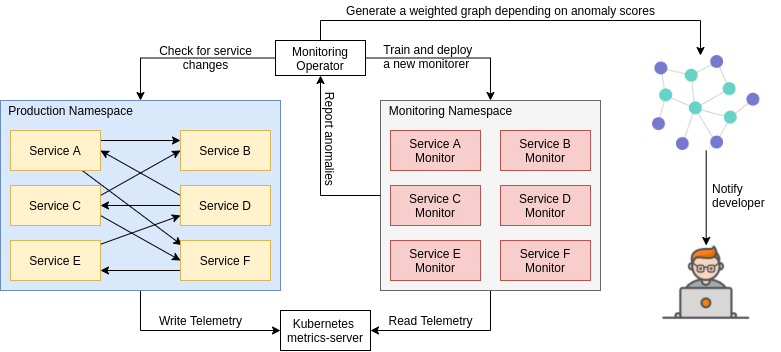
\includegraphics[width=16cm]{assets/High-level-system-diagram.png}
    \caption{High-level system diagram}
    \label{fig:high-level-diagram}
\end{figure}
\section{Research Methodology}
{\let\clearpage\relax \chapter{Development Methodology}}

Even though this project has few clearly defined requirements, designing and developing them will require an iterative model as there isn't a single best way to develop this and the author will be experimenting with different techniques. So author decides on using \textbf{prototyping} as the Software Development Life Cycle Model for this project.

\section{Design Methodology}

To complete this project 2 programming languages need to be used, Python and GoLang. To clean up the dataset and create the model itself Python will be used because most data science tools like TensorFlow and PyTorch were written targeting Python. When it comes to the Kubernetes side, the entire Kubernetes ecosystem was developed using GoLang. Since GoLang doesn't support classes and Python isn't a very OOP-friendly language this project will follow a functional programming paradigm to develop the code-base. 

\section{Evaluation Methodology}

During the literature, the survey author concluded there ain't any specific evaluation metrics for root cause analysis system other than accuracy and f1 score and there ain't any publicly available dataset or a system to benchmark against. But with this research author is hoping to develop a benchmarking system so future researchers can benefit from this.

{\let\clearpage\relax \chapter{Project Management Methodology}}

To manage task of this project authors decide to use \textbf{PRINCE2}. PRINCE2 built upon waterfall method which works best for projects with fixed deadlines and requirements with the added benefit of having regulated inputs and outputs \citep{WhatAreT79:online}.

\section{Deliverables}
\setlength\LTleft{0mm}
\begin{longtable}{|p{115mm}|p{35mm}|}
\hline
\textbf{Deliverable} & \textbf{Date} \\ \hline
\textbf{Draft Project Proposal} & \multirow{2}{*}{02nd September 2021} \\
A draft version of this proposal &  \\ \hline
\textbf{A working beta of MicroSim}\label{microsim} & \multirow{2}{*}{15th September 2021} \\
MicroSim is a tool that simulates a distributed system within a Kubernetes cluster. This tool will be used to test and evaluate the final version of this project &  \\ \hline
\textbf{Research Paper about MircoSim} & \multirow{2}{*}{16th October 2021} \\
MicroSim could have various other use-cases and could help in the development of this research domain. So the author is planning to release it as an open-source project with paper so future research and benefits from this. &  \\ \hline
\textbf{Literature Review Document} & \multirow{2}{*}{21st October 2021} \\
The Document explaining all the existing tools and published researches on the domain &  \\ \hline
\textbf{Project Proposal} & \multirow{2}{*}{04th November 2021} \\
The final version of this project proposal. &  \\ \hline
\textbf{Software Requirement Specification} & \multirow{2}{*}{25th November 2021} \\
The Document all the key requirements that are gonna get address with this research &  \\ \hline
\textbf{Proof of Concept} & \multirow{2}{*}{06th December 2021} \\
Unoptimized prototype with all the main features working &  \\ \hline
\textbf{Interim Progress Report (IPR)} & \multirow{2}{*}{27th January 2022} \\
The document explaining all the preliminary findings and the current state of the project &  \\ \hline
\textbf{Test and Evaluation Report} & \multirow{2}{*}{17th March 2022} \\
A document with results of the project and conclusion made from those tests &  \\ \hline
\textbf{Draft Project Reports} & \multirow{2}{*}{31st March 2022} \\
The draft version of the final thesis &  \\ \hline
\textbf{Final Research Paper} & \multirow{2}{*}{14th April 2022} \\
A paper with results about this project &  \\ \hline
\textbf{Final Project Report} & \multirow{2}{*}{28th April 2022} \\
Finalize version of the thesis &  \\ \hline
\caption{Deliverables and Dates}
\end{longtable}


\newpage
\section{Schedule}
% Gantt chart is a visualization of the task with their respective timelines. Refer Appendix \ref{appendix:gantt-chart} to find the gantt chart for this project.
\begin{figure}[!ht]
    % \chapter{Gantt Chart} \label{appendix:gantt-chart}
    % \centering
    \includegraphics[height=22cm]{assets/gantt-chart.jpg}
\end{figure}


\section{Resource Requirement}

\subsection{Software Requirements}

\begin{itemize}[noitemsep,nolistsep] 
\item \textbf{Linux based operating system} - During this project author will be working with the Kubernetes ecosystem. Most of the Kubernetes tooling are written to work with the Linux kernel.
\item \textbf{Python} - Most of the tooling related to data science like TensorFlow and PyTorch are written as python libraries. Python also provides a lot of help built-in functions to  accelerate the prototyping process.
\item \textbf{GoLang} - Since Kubernetes itself is built using GoLang, It has a very mature client library with a lot of documentation to deal with Kubernetes API.
\item \textbf{Docker and K3d} - To create a Kubernetes cluster locally for development and testing.
\item \textbf{PyCharm and GoLand} - These two are the best IDEs in the market when writing Python and Go projects and it could improve the productivity of developers by big merging. As students, we get a license to use both of those IDEs for free.
\item \textbf{Overleaf / LateX}  - Managing a big document in both MS Word and Google Docs could be a cumbersome task. Especially when adding and removing things both of these software tends to mess up the layout. By using LateX we can declaratively define the layout so it will always behave as intended.
\item \textbf{Google Drive and Github} - Offsite location to backup the codebase and related documents.
\item \textbf{ClickUp} - To manage the project and keep track of things to be done.
\end{itemize}

\subsection{Hardware Requirements}
\begin{itemize}[noitemsep,nolistsep] 
    \item \textbf{A Quad-core CPU with AVX support} - Simulating a distributed system locally will take a lot of processing power. Having an AVX supported CPU will reduce the inference time when testing it on a cluster.
    \item \textbf{GPU with CUDA support and 2GB of VRAM} - Both Tensorflow and Pytorch depend on CUDA for hardware-accelerated training. Training on GPU could save a lot of time increases the number of trial and error iterations that could be done. Having more VRAM could help with building larger models.
    \item \textbf{16 GB Memory} - Running a microservices simulation locally will consume a lot of memory and while testing models will get loaded into RAM. Here having dual-channel memory will be preferable. 
    \item \textbf{20GB disk space} - Models and datasets won't take a lot of disk space but again running the Kubernetes cluster demands a lot of disk space because it needs to keep a lot of containers locally cached.
\end{itemize}

\subsection{Skill Requirements}
\begin{itemize}[noitemsep,nolistsep] 
    \item \textbf{Experience working with Kubernetes} - The author will be developing a Kubernetes extension so they need to know the inner workings of Kubernetes.
    \item \textbf{Data engineering} -  Developing a data encoding technique requires a lot of knowledge in how to manipulate a given dataset.
    \item \textbf{Model engineering} - To complete the project, a completely new model has to be built from the ground up. So the author needs to have an in-depth idea about how to create a model in a machine learning framework and how different layers in the model work to fit them properly. 
\end{itemize}

\subsection{Data Requirements}
\begin{itemize}[noitemsep,nolistsep] 
\item \textbf{Monitoring dataset} -  This dataset can be collected using \hyperref[microsim]{MicroSim} tool author plan to develop to simulate distributed system.
\end{itemize}

\section{Risk Management}


\begin{longtable}{|p{4cm}|p{2cm}|p{2cm}|p{7cm}|}
    \hline
    \textbf{Risk Item} & 
    \textbf{Severity} & 
    \textbf{Frequency} & 
    \textbf{Mitigation Plan}
    \\ \hline
    
    The hypothesis the research is based on is wrong & 
    5 & 
    1 & 
    Present the findings and explain why the hypothesis was wrong 
    \\ \hline
    
    Failure in work computer & 
    4 & 
    3 & 
    Daily backup work the work to a cloud platform 
    \\ \hline
    
    Lack of domain knowledge & 
    2 & 
    3 & 
    Talk to a domain expert, Do more research 
    \\ \hline
    
    Models not generalizing & 
    3 & 
    4 & 
    Explore different methods, Try cleaning up the dataset more 
    \\ \hline
    
    Dataset quality is not up to the standard & 
    4 & 
    1 & 
    Use a method used in related researches to create a new dataset 
    \\ \hline
    
    Running out of time & 
    1 & 
    2 & 
    Have a proper work schedule from the start 
    \\ \hline
    
    Getting sick and unable to work for few days & 
    3 & 
    3 & 
    Keeping few days of a buffer period before deadlines 
    \\ \hline
    \caption{Risks and Mitigation}
\end{longtable}

\cleardoublepage
\phantomsection
\renewcommand{\bibname}{References}
\pagenumbering{Roman}
\setcounter{page}{5}
\addcontentsline{toc}{chapter}{References}
\bibliography{references.bib}

% \begin{appendices}
% \begin{figure}[!ht]
    \chapter{Gantt Chart} \label{appendix:gantt-chart}
    \centering
    \includegraphics[height=22cm]{assets/gantt-chart.png}
\end{figure}
% \end{appendices}

\end{document}

